\section{Introduction}

Remy~\cite{winstein2013tcp} demonstrated that computer-generated congestion
control algorithms could outperform decades of human design within their
training distribution. However, Remy's decision tree CCAs generalize poorly
to network conditions outside their training range. Despite this being
identified over a decade ago, no one has published an apples-to-apples
comparison putting alternative representations on Remy's generalization
graphs---training on the same environments, with the same observation space
and action space.

We set out to add new lines to these graphs. Keeping the observation space
(4~EWMA features), action space (window\_increment, window\_multiple,
intersend), and training environments fixed, we ask: \textbf{how do a neural
network and an LLM-guided code evolution system compare to Remy's decision
trees on out-of-distribution generalization?}

We compare three representations:

\begin{enumerate}
\item \textbf{Decision trees} (Remy): A WhiskerTree maps observation bins to
  actions, optimized by evolutionary search over tree structure.
\item \textbf{Neural networks} (PPO): A PolicyNet with ${\sim}$5000
  parameters maps the same observations to the same actions, trained by
  proximal policy optimization in Remy's C++ simulator.
\item \textbf{Source code} (AlphaCC): GPT-5.3-codex generates Python
  functions that map observations to actions, evolved by LLM-guided mutation
  with simulation-based fitness evaluation.
\end{enumerate}

The third paradigm was not part of the original plan. We added it after
observing that PPO did not beat Remy, and were curious whether an approach
that produces \emph{readable code}---rather than opaque weights---would
generalize differently. In the preserved artifact, the answer is mixed:
AlphaCC reconstructs familiar TCP-like structure and yields readable policies,
but the retained single-point run underperforms Remy and the more robust
hand-designed baselines at most rates. Multi-point training helps sharply in
the best retained run, but the archived results remain high-variance.

\paragraph{Threats to validity.}
Our Python simulator does not exactly replicate Remy's C++ simulator. Small
differences in event scheduling, buffer management, and timing may affect
absolute scores. Cross-method comparisons should be interpreted cautiously
since Remy and PPO were trained in C++ while AlphaCC policies were trained in
Python. The current artifact preserves both C++ evaluation outputs and Python
simulation outputs; we therefore treat cross-method comparisons as qualitative
evidence rather than strict numerical equivalence (\S\ref{sec:calibration}).


\section{Shared Experimental Setup}

\subsection{Remy's Framework}

Remy optimizes a WhiskerTree: a binary decision tree that maps an observation
vector (the ``Memory'') to an action triple. The observation space consists of
four exponentially weighted moving averages (EWMAs):
\begin{itemize}
\item \texttt{send\_ewma}: EWMA of inter-send times ($\alpha = 1/8$)
\item \texttt{rec\_ewma}: EWMA of inter-receive times ($\alpha = 1/8$)
\item \texttt{rtt\_ratio}: smoothed RTT / minimum RTT
\item \texttt{slow\_rec\_ewma}: EWMA of inter-receive times ($\alpha = 1/256$)
\end{itemize}

The action space is:
\begin{itemize}
\item \texttt{window\_increment}: additive change to the congestion window
\item \texttt{window\_multiple}: multiplicative scaling of the congestion window
\item \texttt{intersend}: minimum inter-packet send time (pacing)
\end{itemize}

The utility function for each sender is:
\begin{equation}
U = \log_2(\text{throughput}) - \delta \cdot \log_2(\text{delay})
\end{equation}
where $\delta = 1$. Remy optimizes the sum of sender utilities over a
\texttt{ConfigRange} specifying link rates, delays, and number of senders.

\subsection{Normalized Score}

To compare across link rates, we use a normalized score:
\begin{equation}
S = \log_2\!\left(\frac{\text{throughput}}{\text{capacity}}\right) - \log_2\!\left(\frac{\text{delay}}{\text{min\_rtt}}\right)
\end{equation}
This measures how close a CCA comes to fully utilizing the link (first term)
while keeping delay near the propagation minimum (second term). A score of 0
means perfect utilization with zero queuing delay. All results report
mean $\pm$ standard deviation across 5 random seeds unless noted.

\subsection{Training Condition}

All three methods are trained on a single condition: 1.0 packets/ms link rate
(${\approx}$10~Mbps with 1500-byte packets), 150~ms propagation RTT, 2
senders with Poisson on/off traffic (mean 5s on, 5s off). This matches Remy's
original single-point training configuration. Note: evaluation uses Remy's
original link rates, where 0.946~ppt ($\approx$9.5~Mbps) is the closest
rate to the training condition of 1.0~ppt. For the archived comparison plots,
we use the preserved 30-second evaluation outputs in \texttt{results/}.

\subsection{Fairness Ledger}

The three methods differ on multiple axes beyond representation. We document
these differences so readers can assess which conclusions are attributable to
representation versus other factors.

\begin{table}[t]
\centering
\caption{Fairness ledger: confounds beyond representation.}
\label{tab:fairness}
\small
\begin{tabular}{@{}p{1.6cm}p{1.8cm}p{1.8cm}p{1.8cm}@{}}
\toprule
Factor & Remy & PPO & AlphaCC \\
\midrule
Repr.     & WhiskerTree & Neural net (${\sim}$5K params) & Python source \\
Optimizer & Tree search & PPO & LLM mutation \\
Train sim & C++ (original) & C++ (original) & Python (reimpl.) \\
Budget    & ${\sim}$179K evals & ${\sim}$3M steps & 75 (1pt) / 150 (mpt) \\
Priors    & Obs.\ binning & Reward shaping & Pre-trained TCP knowledge \\
State     & Fixed/region & Hidden state & Arbitrary \\
Variance  & 5 sim seeds & 6 brains & 5 sim seeds \\
\bottomrule
\end{tabular}
\end{table}

\subsection{Evaluation Protocol}

Primary evaluation: 9 link rates spanning 2.4--95~Mbps (a ${\sim}$40$\times$
range), RTT${}={}$150~ms, 2 senders. Extended evaluation: 3 RTT values (50,
150, 300~ms) $\times$ 3 link rates. The archived figure-generation pipeline
uses 30-second runs and the preserved outputs under \texttt{results/python\_sim}
and \texttt{results/cpp\_sim}.

Remy has zero variance in the preserved C++ curves (single deterministic
tree); PPO std is across 6 independently trained brains; Copa, AIMD, and
AlphaCC std are across 5 sim seeds.


%% ====================================================================
%% ANDREW'S SECTION: Simulator Calibration
%% ====================================================================
\subsection{Simulator Calibration}
\label{sec:calibration}

We reimplemented Remy's C++ event-driven simulator in Python, matching the
per-tick event ordering, single-packet-per-sender-per-tick semantics, and
fair-share time accounting from the original C++ source. The retained artifact
includes paired C++ and Python evaluation outputs for several trained
WhiskerTrees. These agree on the broad qualitative picture---narrow trees peak
near their training region, broader trees flatten the curve---but differ
materially in absolute normalized score. We therefore use the calibration as a
sanity check on trend preservation, not as evidence that C++ and Python scores
are numerically interchangeable.


%% ====================================================================
%% ARMAAN'S SECTION: Deep RL Methodology
%% ====================================================================
\section{Deep Reinforcement Learning}
\label{sec:deeprl}

We refactored Remy's C++ simulator to expose a gym-like interface and trained
a PolicyNet (${\sim}$5000 parameters) using proximal policy optimization.
The network maps the same 4D EWMA observations to discretized actions via
three categorical heads (257/101/56 classes for window\_increment,
window\_multiple, and intersend respectively). We trained 6 independent runs
(``brains'') to measure training variance. In the preserved evaluation
artifacts, all 6 PPO brains underperform the 1$\times$ Remy tree across the
9 canonical link rates.


\section{AlphaCC: LLM-Guided Code Evolution}
\label{sec:llm}

\subsection{Evolution Architecture}

Our approach adapts LLM-guided code evolution, inspired by
AlphaEvolve~\cite{alphaevolve2025}, to congestion control. The evolution loop
proceeds as follows:

\begin{enumerate}
\item \textbf{Seed population}: We initialize with five hand-designed CCAs
  implemented as Python functions: AIMD, Copa, an adaptive hybrid, a
  BBR-like estimator, and a pacing-oriented seed.
\item \textbf{Mutation}: GPT-5.3-codex receives the parent policy's source
  code, its fitness score, and the top-performing policies in the archive.
  It generates a mutated policy.
\item \textbf{Evaluation}: The candidate is compiled, sanity-checked (it must
  increase the congestion window when no congestion is detected), and evaluated
  on the training condition.
\item \textbf{Selection}: Parents are chosen with 50\% exploitation (highest
  fitness) and 50\% exploration (random archive member).
\end{enumerate}

We run 15 generations with 5 candidates per generation (75 total evaluations).

\subsection{Policy Representation}

AlphaCC policies are Python functions with the signature:
\begin{verbatim}
def evolved_policy(memory)
\end{verbatim}
where \texttt{memory} is Remy's Memory (4 EWMAs) and the return value is Remy's
Action triple (window\_increment, window\_multiple, intersend). Policies can
maintain state across calls via function attributes (e.g.,
\texttt{evolved\_policy.phase}), enabling stateful behaviors like phase
transitions and bandwidth estimation.

\subsection{Observed Structural Patterns}

Across the retained single-point archive, viable policies repeatedly use some
combination of:
\begin{itemize}
\item \textbf{AIMD}: Additive increase / multiplicative decrease as the
  core control loop.
\item \textbf{Slow start}: Exponential window growth until RTT inflation is
  detected (\texttt{rtt\_ratio} $>$ 1.25).
\item \textbf{Rate estimation}: Using \texttt{rec\_ewma} as a bandwidth proxy
  to set pacing rates.
\item \textbf{Pacing}: Setting \texttt{intersend} based on estimated available
  bandwidth.
\end{itemize}

None of these mechanisms are provided as executable templates. The model
reconstructs them from pre-trained knowledge and from the surviving policies in
the archive. Whether this is a helpful structural prior or a source of
architectural lock-in is one of the central questions in
Section~\ref{sec:ablation}.

Note that AlphaCC policies can maintain arbitrary state across calls via function
attributes (e.g., phase tracking, bandwidth estimates), which is additional
representational power not available to Remy's fixed tree mapping or PPO's
fixed-size hidden state. The statefulness ablation (\S\ref{sec:ablation})
partially addresses this confound.


\section{Results}
\label{sec:results}

\subsection{Generalization Across Link Rates}

Figure~\ref{fig:generalization} and Table~\ref{tab:generalization} show the
normalized score for all methods across 9 link rates spanning 2.4--95~Mbps.

\begin{figure}[t]
\centering
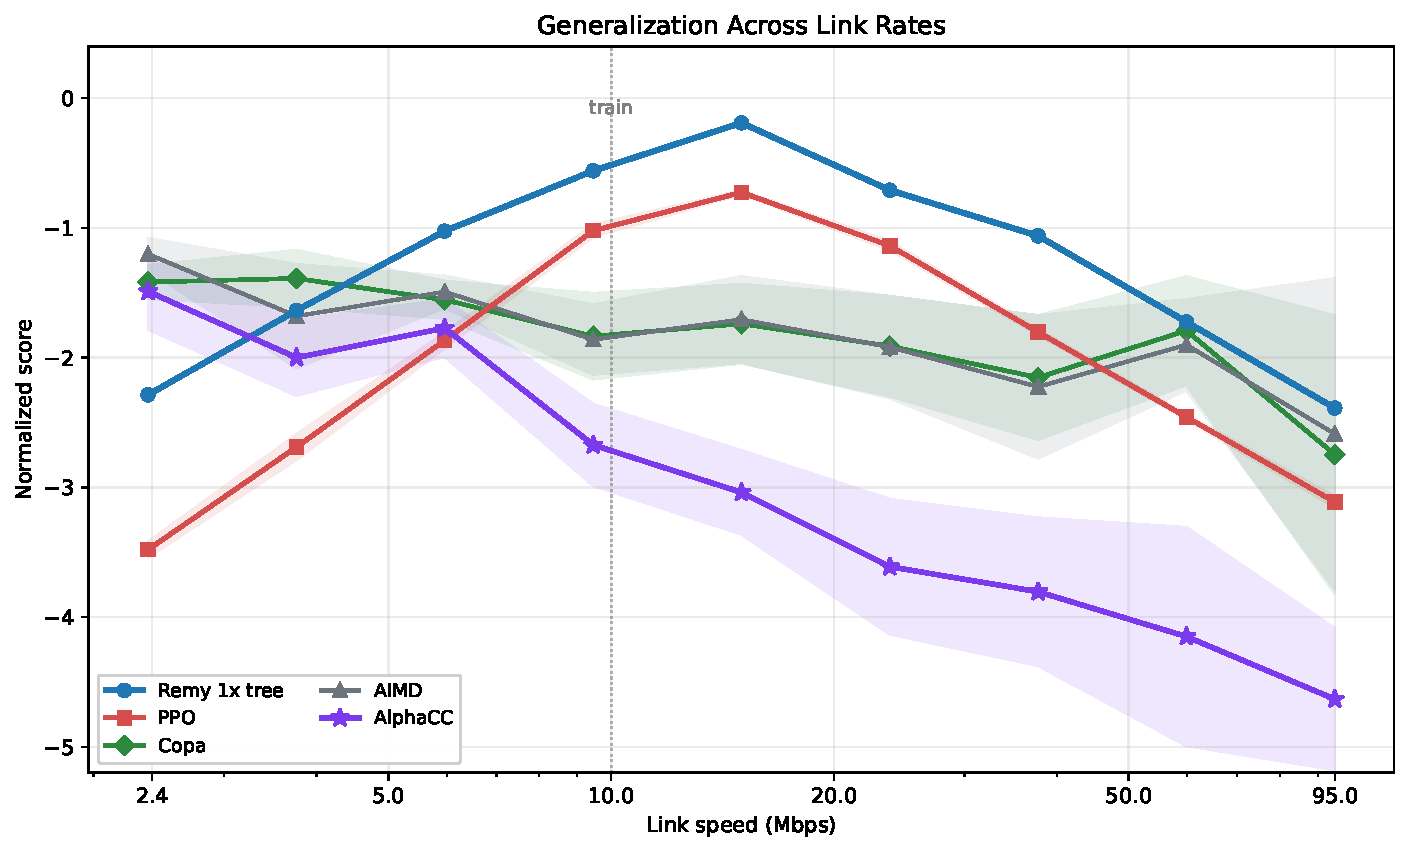
\includegraphics[width=\columnwidth]{figures/fig1_generalization_v2}
\caption{Normalized score vs.\ link rate. Remy peaks near training (15~Mbps)
but degrades at both extremes. PPO stays below Remy at every tested rate.
Copa and AIMD are flatter than the retained single-point AlphaCC run, whose
curve degrades sharply as link rate increases. Shaded bands: PPO range
(6 brains) and AlphaCC $\pm$1$\sigma$ (5 seeds).}
\label{fig:generalization}
\end{figure}

\begin{table}[t]
\centering
\caption{Normalized score (mean $\pm$ std) across 9 link rates. Bold marks
the best mean at each rate. Remy: single deterministic tree;
PPO: std across 6 brains.}
\label{tab:generalization}
\small
\begin{tabular}{@{}rrrrrr@{}}
\toprule
Mbps & Remy & PPO & Copa & AIMD & AlphaCC \\
\midrule
2.4  & $-$2.29 & $-$3.48{\scriptsize$\pm$.06} & $-$1.42{\scriptsize$\pm$.13} & \textbf{$-$1.20}{\scriptsize$\pm$.12} & $-$1.49{\scriptsize$\pm$.29} \\
3.8  & $-$1.64 & $-$2.69{\scriptsize$\pm$.10} & \textbf{$-$1.39}{\scriptsize$\pm$.22} & $-$1.68{\scriptsize$\pm$.40} & $-$2.00{\scriptsize$\pm$.29} \\
6.0  & \textbf{$-$1.03} & $-$1.87{\scriptsize$\pm$.06} & $-$1.55{\scriptsize$\pm$.14} & $-$1.49{\scriptsize$\pm$.12} & $-$1.77{\scriptsize$\pm$.22} \\
9.5  & \textbf{$-$0.56} & $-$1.02{\scriptsize$\pm$.05} & $-$1.84{\scriptsize$\pm$.33} & $-$1.86{\scriptsize$\pm$.27} & $-$2.67{\scriptsize$\pm$.31} \\
15.0 & \textbf{$-$0.19} & $-$0.73{\scriptsize$\pm$.01} & $-$1.74{\scriptsize$\pm$.30} & $-$1.71{\scriptsize$\pm$.33} & $-$3.04{\scriptsize$\pm$.32} \\
23.8 & \textbf{$-$0.71} & $-$1.14{\scriptsize$\pm$.03} & $-$1.91{\scriptsize$\pm$.38} & $-$1.92{\scriptsize$\pm$.39} & $-$3.61{\scriptsize$\pm$.52} \\
37.7 & \textbf{$-$1.06} & $-$1.80{\scriptsize$\pm$.02} & $-$2.15{\scriptsize$\pm$.48} & $-$2.23{\scriptsize$\pm$.55} & $-$3.80{\scriptsize$\pm$.57} \\
59.8 & \textbf{$-$1.72} & $-$2.46{\scriptsize$\pm$.02} & $-$1.79{\scriptsize$\pm$.42} & $-$1.90{\scriptsize$\pm$.35} & $-$4.15{\scriptsize$\pm$.84} \\
94.9 & \textbf{$-$2.39} & $-$3.11{\scriptsize$\pm$.04} & $-$2.75{\scriptsize$\pm$1.07} & $-$2.59{\scriptsize$\pm$1.20} & $-$4.63{\scriptsize$\pm$.54} \\
\bottomrule
\end{tabular}
\end{table}

Remy peaks at 15~Mbps ($-$0.19) but degrades to $-$2.39 at 95~Mbps,
reproducing the overfitting pattern from the original
paper~\cite{winstein2013tcp}. PPO underperforms Remy at every tested link
rate; this may reflect our training recipe rather than a fundamental RL
limitation, but it is the retained result. Copa and AIMD are materially flatter
across the full range than the retained single-point AlphaCC run. On the
9-point mean metric, AlphaCC is worst overall ($-$3.02) and has the largest
across-rate spread, indicating that readable code alone did not solve the
generalization problem in the single-point setting.

\subsection{Generalization Across RTT}

Figure~\ref{fig:rtt} shows performance across 3 RTT values $\times$ 3 link
rates. Table~\ref{tab:rtt} reports the scores.

\begin{figure}[t]
\centering
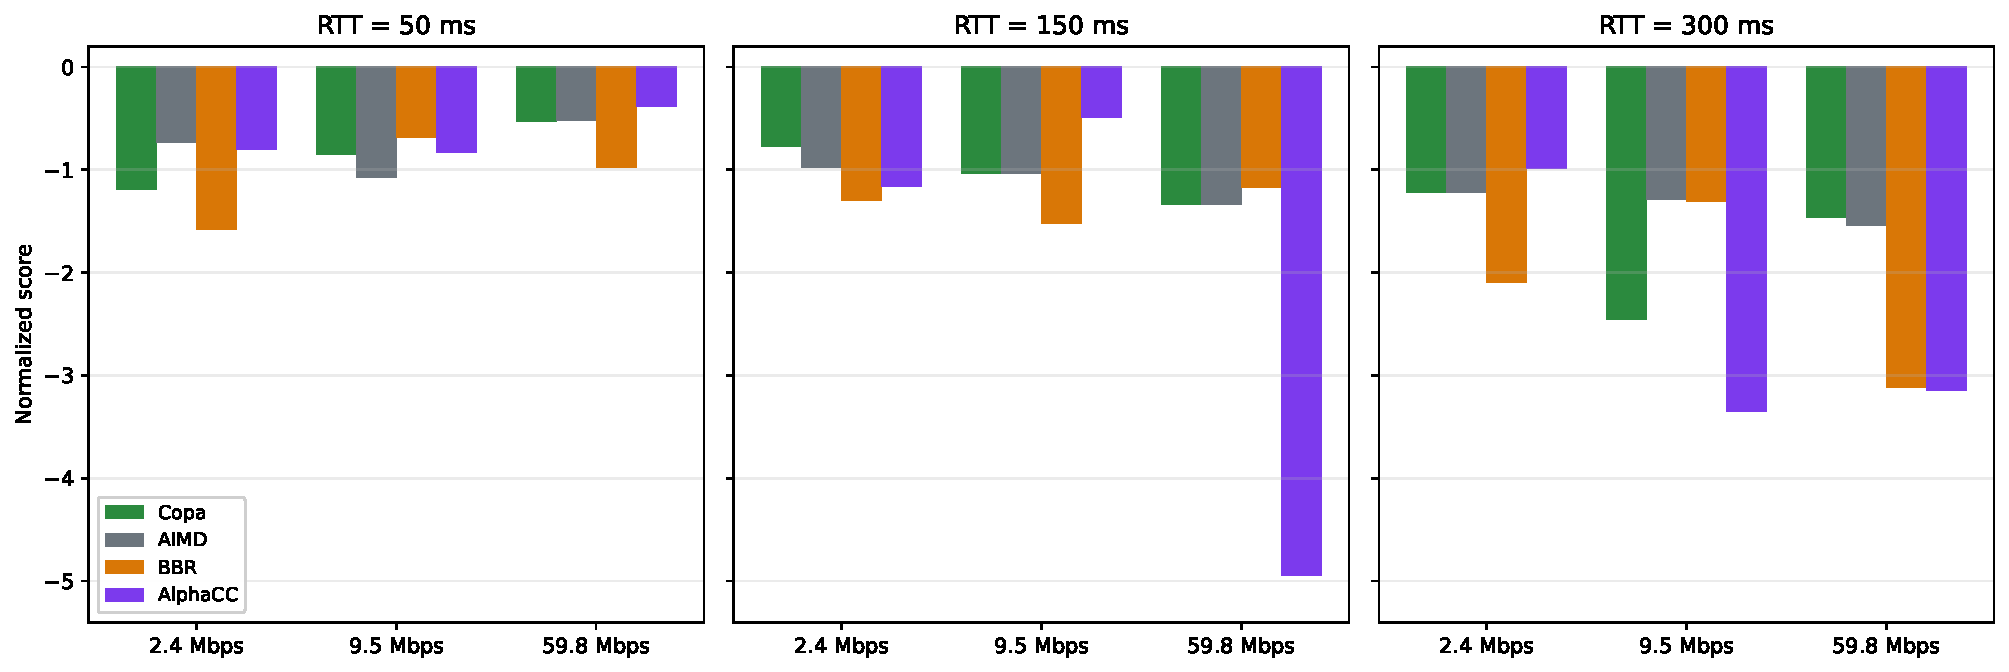
\includegraphics[width=\columnwidth]{figures/fig2_rtt_sweep}
\caption{Normalized score across RTT values (50, 150, 300~ms) and link rates
(2.4, 9.5, 59.8~Mbps). No method dominates all 9 conditions. AlphaCC has two
strong cells, but also one catastrophic failure at 150~ms / 59.8~Mbps.}
\label{fig:rtt}
\end{figure}

\begin{table}[t]
\centering
\caption{RTT sweep results. Single evaluation per condition. Bold marks the
best score per row.}
\label{tab:rtt}
\small
\begin{tabular}{@{}lrrrr@{}}
\toprule
Condition & Copa & AIMD & BBR & AlphaCC \\
\midrule
50ms, 2.4 Mbps        & $-$1.19 & \textbf{$-$0.73} & $-$1.58 & $-$0.80 \\
150ms, 2.4 Mbps       & \textbf{$-$0.77} & $-$0.97 & $-$1.30 & $-$1.16 \\
300ms, 2.4 Mbps       & $-$1.22 & $-$1.22 & $-$2.10 & \textbf{$-$0.99} \\
50ms, 9.5 Mbps        & $-$0.85 & $-$1.08 & \textbf{$-$0.69} & $-$0.83 \\
150ms, 9.5 Mbps       & $-$1.03 & $-$1.03 & $-$1.52 & \textbf{$-$0.49} \\
300ms, 9.5 Mbps       & $-$2.46 & \textbf{$-$1.29} & $-$1.31 & $-$3.35 \\
50ms, 59.8 Mbps       & $-$0.53 & $-$0.52 & $-$0.98 & \textbf{$-$0.38} \\
150ms, 59.8 Mbps      & $-$1.34 & $-$1.34 & \textbf{$-$1.17} & $-$4.94 \\
300ms, 59.8 Mbps      & \textbf{$-$1.46} & $-$1.54 & $-$3.12 & $-$3.15 \\
\bottomrule
\end{tabular}
\end{table}

The RTT sweep reinforces the same pattern as the link-rate sweep: AlphaCC can
produce sharp wins on isolated conditions ($-$0.49 at 150~ms / 9.5~Mbps and
$-$0.38 at 50~ms / 59.8~Mbps), but its tails are poor. No method is uniformly
best across all 9 cells, and the robust hand-designed baselines remain much
more predictable than the retained single-point AlphaCC policy.

\subsection{Throughput-Delay Tradeoff}

Figure~\ref{fig:scatter} shows the throughput-delay tradeoff at the training
condition (0.946~ppt, all methods evaluated consistently).

\begin{figure}[t]
\centering
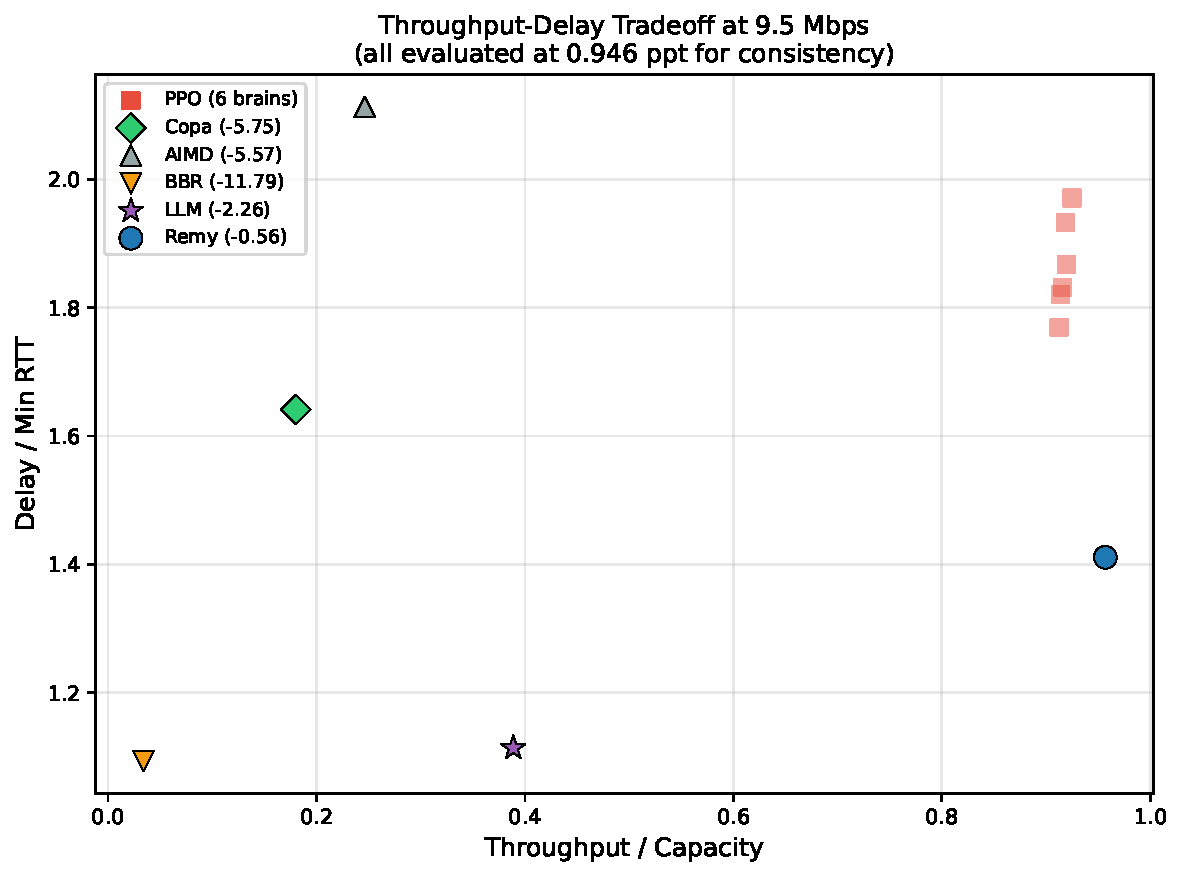
\includegraphics[width=\columnwidth]{figures/fig3_scatter_v2}
\caption{Throughput vs.\ delay at the training condition (9.5~Mbps). Remy and
PPO occupy the high-throughput / higher-delay region. Copa and AIMD are more
delay-conservative. The retained AlphaCC point lands between these extremes
rather than defining a new Pareto frontier.}
\label{fig:scatter}
\end{figure}

The scatter plot is best read qualitatively. Remy remains the strongest
training-point optimizer, PPO tends to buy throughput with more delay, and the
retained AlphaCC policy does not dominate either frontier.

\subsection{Multipoint Training}
\label{sec:multipoint}

The single-point AlphaCC degrades badly at high link rates because it never
encounters them during training. We therefore also retained a multi-point run
trained across 6 link rates with 30 generations, 5 candidates per generation,
and per-rate feedback in the prompt. Figure~\ref{fig:multipoint} shows that the
best preserved multi-point run is dramatically flatter than the retained
single-point run.

\begin{table}[t]
\centering
\caption{Multi-point AlphaCC summary. Mean normalized score across the
9 canonical link rates. C++ and Python rows are shown together only for
qualitative comparison.}
\label{tab:multipoint}
\small
\begin{tabular}{@{}lr@{}}
\toprule
Method & 9-pt Mean \\
\midrule
AlphaCC, single-point (Python) & $-$3.02 \\
AlphaCC, best preserved multi-point run (Python) & \textbf{$-$0.76} \\
AlphaCC, other archived multi-point runs (Python) & $-$1.39 to $-$6.14 \\
Remy 1$\times$ tree (C++) & $-$1.29 \\
Remy 10$\times$ tree (C++) & $-$0.94 \\
\bottomrule
\end{tabular}
\end{table}

The strongest preserved multi-point run improves the 9-point mean score from
$-$3.02 to $-$0.76, a large improvement over the retained single-point run and
competitive with the wider Remy baselines on this archived metric. At the same
time, the other saved multi-point runs still span means from $-$1.39 down to
$-$6.14. Multi-point training helps, but it does not remove the search
instability.

\begin{figure}[t]
\centering
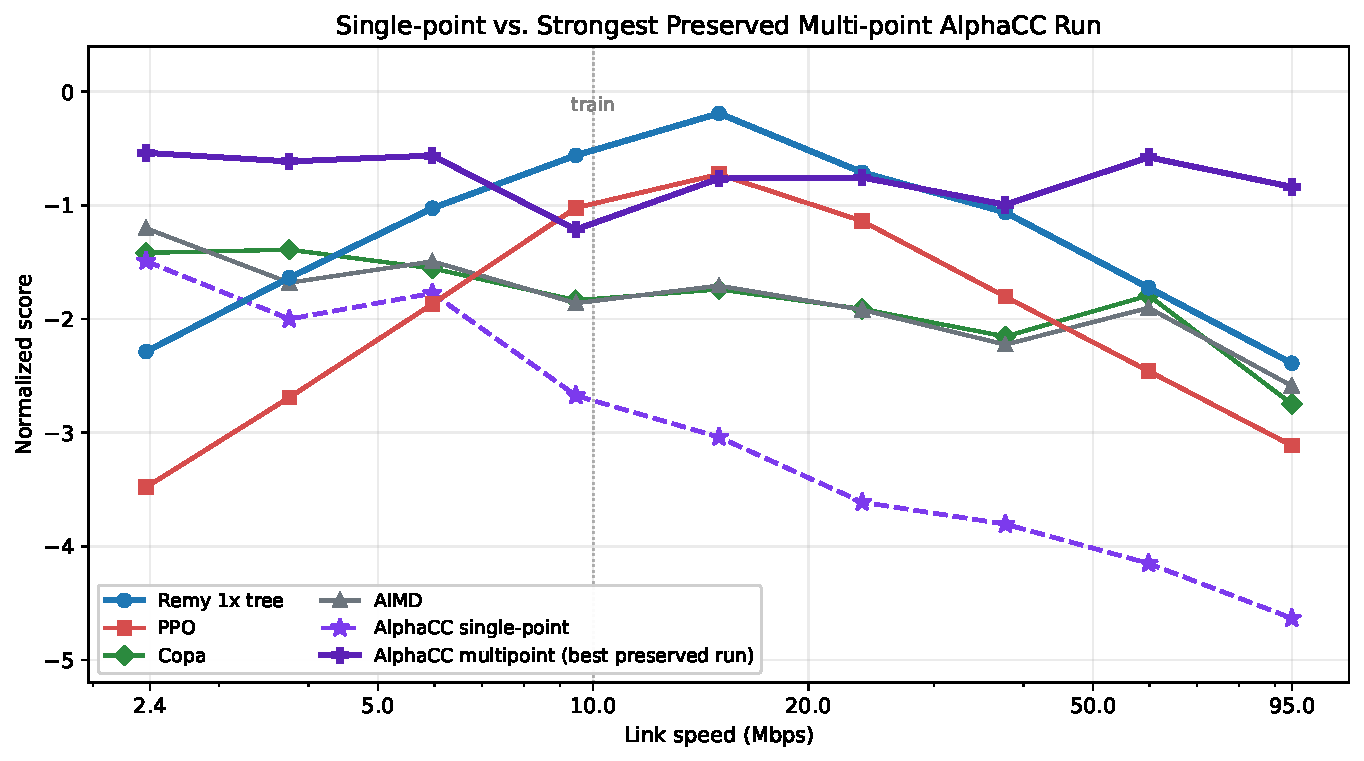
\includegraphics[width=\columnwidth]{figures/fig5_multipoint}
\caption{Best preserved multi-point AlphaCC run (solid) vs retained
single-point AlphaCC (dashed) and Remy baselines. Training across 6 rates
substantially flattens the AlphaCC curve.}
\label{fig:multipoint}
\end{figure}

The strongest preserved multi-point policy converges on a more explicitly
rate-aware architecture than the single-point run, with three recurring
mechanisms:

\begin{enumerate}
\item \textbf{Larger additive growth at higher inferred BDP}: the update rule
  scales more aggressively with estimated bandwidth-delay product than the
  retained single-point policy.
\item \textbf{Continuous pacing}: \texttt{intersend} is tied directly to a
  receive-rate estimate,
  tracking bottleneck rate at any capacity.
\item \textbf{Phase-based probing}: the policy alternates between more and less
  aggressive pacing phases rather than using a single fixed gain everywhere.
\end{enumerate}

\subsection{Ablation: Statefulness}
\label{sec:ablation}

To test whether AlphaCC's extra representational freedom is carrying the
result, we compared the retained stateful single-point policy to a preserved
stateless run in which each action depends only on the current observations
(no function attributes). Table~\ref{tab:ablation} does \emph{not} support a
simple ``more state is better'' story: in the archived runs, the stateless
policy is slightly better at the sampled points, though both are worse than the
hand-designed baselines at most rates.

\begin{table}[t]
\centering
\caption{Statefulness ablation. Stateful and Copa: mean $\pm$ std over 5
seeds. Stateless: single evolution run, best policy.}
\label{tab:ablation}
\small
\begin{tabular}{@{}lrrr@{}}
\toprule
Condition & AlphaCC (stateful) & AlphaCC (stateless) & Copa \\
\midrule
Near-train (9.5 Mbps) & $-$2.67{\scriptsize$\pm$.31} & \textbf{$-$2.54} & $-$1.84{\scriptsize$\pm$.33} \\
Low (2.4 Mbps) & $-$1.49{\scriptsize$\pm$.29} & \textbf{$-$0.75} & $-$1.42{\scriptsize$\pm$.13} \\
High (59.8 Mbps) & $-$4.15{\scriptsize$\pm$.84} & \textbf{$-$1.92} & $-$1.79{\scriptsize$\pm$.42} \\
\bottomrule
\end{tabular}
\end{table}

\subsection{Failure Modes of AlphaCC}
\label{sec:failures}

The archived single-point and multi-point runs reveal recurring failure modes:

\begin{enumerate}
\item \textbf{Architectural lock-in}: early seed choices constrain the later
  search trajectory. Once a lineage commits to a particular controller shape,
  later mutations mostly retune coefficients rather than discovering a new
  design family.
\item \textbf{Over-complex control laws}: some archived runs grow into
  coefficient-heavy PID-like policies whose interacting terms are difficult to
  tune within a 30-generation budget.
\item \textbf{Degenerate mutations}: a few archived runs fall into very poor
  regions of the search space and never recover, indicating that the mutation
  loop behaves more like local search over seeded architectures than like a
  globally exploratory optimizer.
\end{enumerate}

These failure modes suggest that AlphaCC is fundamentally
\emph{local search}---effective within an architecture, but unable to make the
qualitative jumps needed when the initial architecture is wrong.

\subsection{Evolution Trajectory}

Figure~\ref{fig:evolution} shows the evolution trajectory over 15 generations.

\begin{figure}[t]
\centering
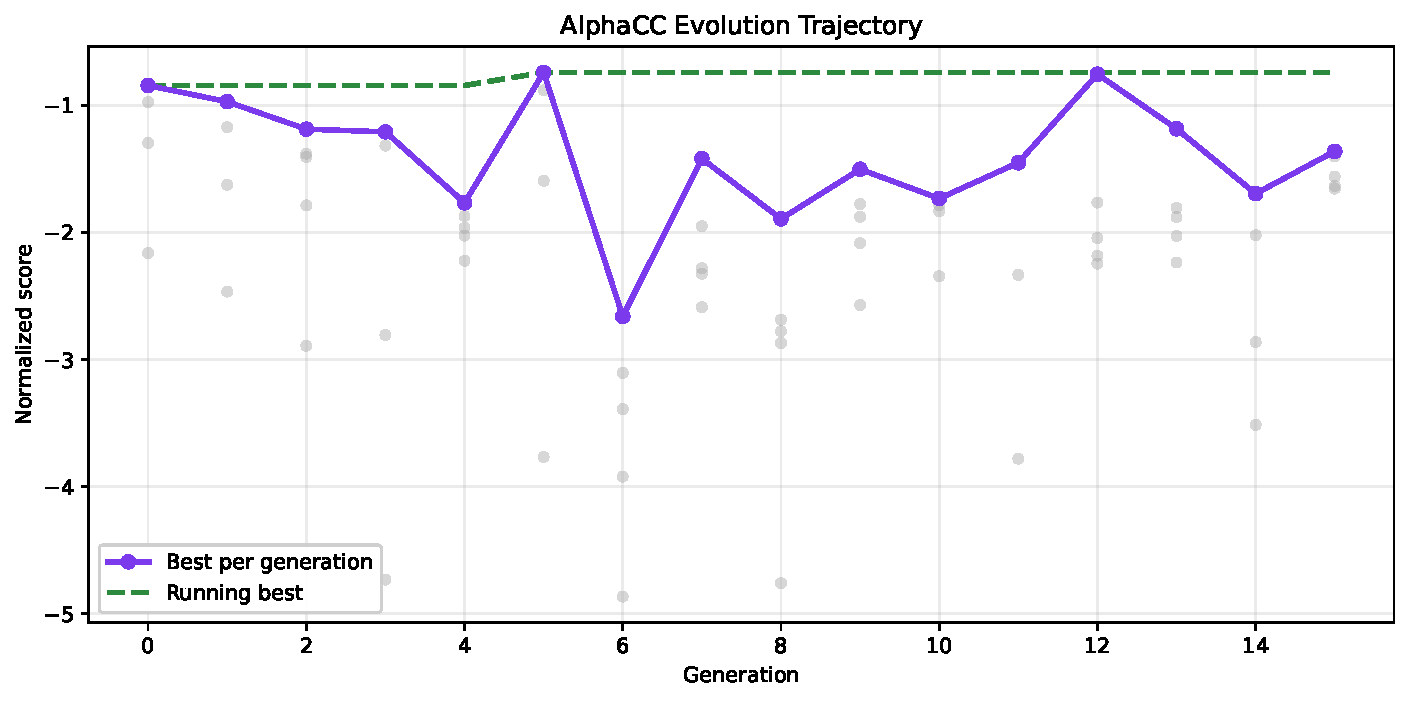
\includegraphics[width=\columnwidth]{figures/fig4_evolution_v2}
\caption{AlphaCC evolution trajectory. Gray dots: all candidates; purple:
best per generation; green dashed: running best. Most improvement occurs
in the first 5 generations.}
\label{fig:evolution}
\end{figure}

Most improvement occurs in the first 5 generations, with diminishing returns
afterward. The best policy emerges from a Copa seed lineage that accumulates
bandwidth estimation, pacing, and phase-transition mechanisms through
successive mutations.


\section{Discussion}
\label{sec:discussion}

\subsection{What the Comparison Shows}

Our results are consistent with the hypothesis that representation affects
generalization, but we cannot isolate representation as the causal factor---the
three methods also differ in optimization budget and training algorithm
(Table~\ref{tab:fairness}).

What the evidence supports:
\begin{itemize}
\item AlphaCC reconstructs known CCA architectures without prompting,
  suggesting strong inductive bias from pre-trained TCP knowledge.
\item This bias is a double-edged sword: sensible designs near training, but
  constrained exploration far from it.
\item Hand-designed CCAs remain competitive, suggesting the bottleneck is
  structural knowledge, not optimization power.
\item Multi-point AlphaCC can dramatically improve over the retained
  single-point run, but the archived outcomes remain high-variance and strongly
  dependent on the seed lineage.
\end{itemize}

The retained single-point AlphaCC policy appears over-specialized to its narrow
training regime. Its control logic adapts too slowly as capacity grows, and the
resulting curve collapses at the upper end of the 40$\times$ sweep. Multi-point
training partly fixes this by forcing the policy to experience a broader range
of bandwidth-delay products during evolution.

\subsection{Interpretability}

AlphaCC's unique property is that its output is human-readable code.
The retained best single-point policy is 105 lines of Python with named
variables and clear
control flow; PPO's equivalent is ${\sim}$5000 opaque weights. This means
AlphaCC's output can be directly inspected, debugged, and understood by a
networking engineer---enabling the mechanism analysis in
Section~\ref{sec:multipoint} that would be impossible with a neural network.

\subsection{Limitations}

\begin{enumerate}
\item \textbf{PPO baseline quality}: Our PPO results may reflect suboptimal
  hyperparameters rather than a fundamental RL limitation.
\item \textbf{Simulator mismatch}: Remy/PPO results are preserved from C++
  artifacts, while AlphaCC runs in the Python reimplementation. Absolute
  cross-method scores are therefore only qualitatively comparable.
\item \textbf{Prior injection}: AlphaCC evolution uses hand-designed seeds and
  prompt guidance. The resulting policies are not ``from scratch'' search.
\item \textbf{Archived multi-point variance}: the saved multi-point runs span
  very strong and very poor outcomes, so the evidence supports possibility, not
  reliability.
\item \textbf{No stochastic loss}: All experiments use lossless links.
\item \textbf{Simulator only}: No Mahimahi or real-network validation.
\end{enumerate}


\section{Related Work}

Remy~\cite{winstein2013tcp} pioneered automated CCA design with decision tree
optimization. Sivaraman et al.~\cite{sivaraman2014experimental} studied its
generalization, finding that trees trained on narrow ranges degrade on wider
conditions but that very wide training ranges (1000$\times$) achieve
within-3\% throughput of narrow-range trees.

Several deep RL approaches followed: PCC~\cite{dong2015pcc} used online
learning for utility maximization; Aurora~\cite{jay2019deep} applied deep RL
to congestion control; Yan et al.~\cite{yan2018pantheon} built the Pantheon
benchmarking platform and trained Indigo via imitation learning.
These demonstrated that neural networks can learn congestion control but
did not systematically compare generalization across representations on the
same environments.

CCAC~\cite{arun2021ccac} introduced formal verification of CCAs using SMT
solvers. CCmatic~\cite{arun2024ccmatic} extended this to automated synthesis
with formal guarantees, but within a fixed cwnd-adjustment template.

AlphaEvolve~\cite{alphaevolve2025} demonstrated LLM-guided code evolution for
mathematical optimization. Our approach adapts this paradigm to congestion
control, using simulation-based fitness instead of mathematical verification.

Copa~\cite{arun2018copa} and BBR~\cite{cardwell2017bbr} represent hand-designed
CCAs that encode domain knowledge about delay-based and model-based congestion
control, respectively.


\section{Conclusion}

We set out to put new lines on Remy's generalization graphs---training a
neural network and AlphaCC on the same environments,
with the same observations and actions. Our findings:

\begin{enumerate}
\item \textbf{The generalization problem persists.} Neither PPO nor AlphaCC
  evolution consistently outperforms Remy near its training condition. All
  automatically generated CCAs degrade outside their training distribution.

\item \textbf{PPO is inconclusive.} In our implementation, PPO underperforms
  Remy at every link rate. This may reflect our training recipe rather than a
  fundamental limitation, but it is the result we have.

\item \textbf{AlphaCC is high-variance but interpretable.} With
  multi-point training, the best retained run improves sharply over the
  single-point run and approaches the narrower Remy 1$\times$ baseline at
  several rates. But the saved runs remain highly unstable, with several
  collapsing into poor local minima.

\item \textbf{Hand-designed structure transfers best.} Copa and AIMD show
  the flattest generalization curves, suggesting the bottleneck in automated
  CCA design is structural knowledge, not optimization power. AlphaCC's
  pre-trained TCP knowledge gives it structural priors that PPO
  lacks---but these priors constrain as much as they help.
\end{enumerate}
